\documentclass[conference,letterpaper,10pt]{IEEEtran}
\usepackage[T1]{fontenc}
\usepackage{cite}
\usepackage{amsmath,amssymb,amsfonts}
\usepackage{amsthm}
\usepackage{graphicx}
\usepackage{array,booktabs}
\usepackage{tikz}
\usepackage{tcolorbox}
\tcbuselibrary{breakable,skins}
\usepackage{url}
\usepackage[hidelinks]{hyperref}

\newtheorem{definition}{Definition}
\newtheorem{theorem}{Theorem}
\newtheorem{lemma}{Lemma}
\newtcolorbox[auto counter,number within=section]{myframebox}[1][]{
  colback=white,colframe=black!80,width=\linewidth,
  boxrule=0.5pt,arc=1mm,breakable,
  fonttitle=\bfseries,coltitle=black,
  colbacktitle=white,title=Functionality \thetcbcounter,
  left=4pt,right=4pt,top=3pt,bottom=3pt,boxsep=0pt,
  #1
}

\begin{document}
\title{Composable Security and Conditional Termination of Tendermint}
\author{\IEEEauthorblockN{Regular Paper}}
\maketitle

\begin{abstract}
We study an abstract Tendermint consensus specification in the Generalized Universal Composability framework. An operational ideal service captures consensus transitions using session-local communication and timers and a shared reference clock. Under fixed voting weights and static Byzantine weight below one third, we present execution correspondence, weighted-quorum and lock-safety arguments, and an event-by-event simulation argument. We separately derive a conditional post-stabilization latency bound for exact timers, zero local processing, and immediate activation service. The bound accounts for quorum-triggered waits, proposer and lock-evidence fairness, and the starting round and its entry time. The numerical fairness bound is not inferred from stake weights alone. Bounded TLA+ checks are supplementary evidence and do not establish UC realization or unbounded termination.
\end{abstract}
\begin{IEEEkeywords}
Tendermint, Byzantine fault tolerance, universal composability, conditional termination, formal verification
\end{IEEEkeywords}

\section{Introduction}\label{sec:introduction}

Modern blockchain systems operate in decentralized, adversarial environments where network delays and malicious actors challenge protocol correctness and progress. Byzantine Fault-Tolerant (BFT) protocols originated from the formulation of the Byzantine Generals Problem~\cite{lamport1982byzantine}. In weighted consensus, the relevant fault condition is stated in voting power rather than validator count. To reflect real-world conditions, the partially synchronous model~\cite{dwork1988consensus} and PBFT~\cite{castro1999practical} use a Global Stabilization Time (GST), after which honest-to-honest message delivery is bounded.

Subsequent research has focused on improving efficiency and reducing latency through diverse mechanisms. SBFT~\cite{gueta2019sbft} achieves sub-quadratic complexity via threshold signatures, while HotStuff~\cite{yin2019hotstuff} and Tendermint~\cite{kwon2014tendermint,buchman2018latest} utilize linear communication and locking mechanisms to support large-scale deployments. Modularity is further enhanced in Hyperledger Fabric~\cite{androulaki2018hyperledger} by decoupling consensus from execution. Recent designs continue to minimize commit latency or leverage Directed Acyclic Graph (DAG) structures, where Jolteon~\cite{gelashvili2022jolteon} employs a linear two-chain path, HotStuff-2~\cite{malkhi2023hotstuff} enables optimistic two-phase commits, and DAG-Rider~\cite{keidar2021all} maximizes throughput in asynchronous settings.

Among these protocols, Tendermint represents a widely adopted and practically efficient BFT consensus mechanism, underpinning major platforms such as Cosmos~\cite{kwon2019cosmos}, BNB Chain~\cite{bnbchain2020whitepaper}, Oasis Network~\cite{oasis2020whitepaper}, and IRISnet~\cite{irisnet2018whitepaper}.

Initially proposed by Kwon~\cite{kwon2014tendermint} and later formalized by Buchman et al.~\cite{buchman2018latest}, Tendermint integrates a gossip-based peer-to-peer communication layer to improve efficiency.
Existing research provides a foundation for the correctness of Tendermint. Amoussou-Guenou et al.~\cite{amoussou2018correctness} formalize the security properties of Tendermint to show that a modified version achieves one-shot consensus under eventual synchrony. Subsequently, Roughgarden~\cite{roughgarden2021lecture7} identifies and proves three core mechanisms: repeated single-shot consensus, timeout-driven round progression, and a two-stage voting process. These elements ensure a two-thirds supermajority forms a quorum certificate, which maintains safety under Byzantine faults.

Despite these advances, existing analyses primarily focus on standalone correctness under isolated network assumptions. While such approaches establish safety and eventual termination in isolation, providing formal security guarantees for modular interactions with other components, such as access control and cross-chain protocols, remains a significant challenge in concurrent settings.

To address these limitations, we adopt the Universal Composability (UC) framework~\cite{canetti2001universally}, which models security via an ideal-world/real-world paradigm. In this framework, the protocol is abstracted as an ideal functionality $\mathcal{F}_{ \scriptscriptstyle \mathsf{Tendermint}}$ that captures its desired properties independently of implementation details. Security is defined through indistinguishability: no environment $\mathcal{Z}$ can distinguish between executions in the real and ideal worlds.

The UC composition theorem transfers simulation-based security under its stated setup and interface conditions; it does not by itself imply a termination bound. Beyond consensus, UC has been used to formalize secure multi-party computation~\cite{canetti2002universally}, secure communication channels~\cite{canetti2002universallykeyexchange}, digital signatures~\cite{canetti2004universally}, commitment schemes~\cite{canetti2001universallycommitments}, and zero-knowledge proofs~\cite{camenisch2011framework}.

The UC framework requires a precise ideal service and resource interfaces; it does not prohibit stateful functionalities. We retain operational phase and lock guards in the ideal service and relate them to the real protocol through execution correspondence. The existing TLA$^+$ artifact is a separate bounded transition-system analysis; its results are not used as a proof of the UC statement or unbounded liveness.

Founded on the unification of state-transition systems and temporal reasoning introduced by Lamport~\cite{lamport1994temporal,lamport1999specifying}, TLA+ provides a rigorous framework for modeling concurrent and distributed systems, and is well suited for our purpose.

Prior work formally studies Tendermint synchronization and light-client protocols~\cite{braithwaite2020formal,braithwaite2020tendermint}. The TLA$^+$ section retained from the original manuscript reports bounded checks of its executable transition model; those checks are supplementary and do not establish the GUC or liveness claims made here.

\subsection{Our Contributions}\label{sec:contributions}

Dong et al.~\cite{dong2025uctendermint} present a UC analysis of Tendermint. The present treatment makes explicit the operational ideal service, weighted quorum guards, resource interfaces, and conditions of the simulation and timing arguments.

\begin{itemize}
    \setlength{\itemsep}{0pt}
    \setlength{\parsep}{0pt}
    \setlength{\topsep}{2pt}
    \item We specify an operational ideal functionality and a corresponding Tendermint protocol, with voting power fixed within each height and round-dependent proposer selection.

    \item We state the GUC simulation claim in the hybrid model with session-local public communication and timers and a shared reference clock, and give an event-by-event internal-simulation argument for static corruption.

    \item Under Byzantine voting weight $W_B<W/3$, gossip and timing premises, and explicit proposer/lock-evidence fairness, we give a conditional latency bound in the exact-timer, zero-local-processing specialization. The bound includes quorum-triggered waiting and retains the starting round and its entry time.

    \item The paper also reports the original bounded TLA$^+$ checks as supplementary executable evidence; these checks are not used to prove the UC realization or the unbounded liveness result.

\end{itemize}

The results concern the cited abstract Tendermint specification and do not claim verification of a particular ChainMaker release or implementation.

\subsection{Organization} \label{sec:organization}

The remainder of the paper is organized as follows. Section~\ref{sec:preliminaries} introduces UC/GUC and the abstract Tendermint consensus rules. Section~\ref{sec:model} defines the operational functionality, local hybrid interfaces, and global reference clock. Section~\ref{sec:protocol} gives the protocol model, simulation argument, weighted safety reasoning, and conditional post-GST liveness bound. Section~\ref{sec:tla+} reports the bounded TLA$^+$ analysis retained from the original manuscript; it is separate from the UC proof. Section~\ref{sec:conclusion} summarizes the scope and limitations.

\section{Preliminaries}\label{sec:preliminaries}

This section reviews the UC and Generalized UC (GUC) security frameworks, the Tendermint protocol, and TLA+ for formal modeling and verification.

\subsection{Universally Composable Security}

The Universally Composable (UC) framework~\cite{canetti2001universally} ensures protocol security under concurrent composition by modeling participants, adversaries, and ideal functionalities as Interactive Turing Machines (ITMs). For precise session isolation, each ITM instance (ITI) is uniquely identified by a pair $(\mathsf{pid}, \mathsf{sid})$. ITIs interact via specialized tapes: input and output for messages, subroutine for functionalities, and backdoor for adversarial coordination.

The UC framework enables modular analysis via its composition theorem and supports expressive adversarial models. Beyond consensus, UC has been used to formalize secure multi-party computation~\cite{canetti2002universally}, secure communication channels~\cite{canetti2002universallykeyexchange}, digital signatures~\cite{canetti2004universally}, commitment schemes~\cite{canetti2001universallycommitments}, and zero-knowledge proofs~\cite{camenisch2011framework}.

\subsubsection{The GUC Framework}

Security in the UC framework is defined by simulation: for every adversary $\mathcal{A}$ there must be a simulator $\mathcal{S}$ such that no allowed environment distinguishes real from ideal execution. GUC~\cite{canetti2007universally} additionally models globally shared setup functionalities. A global functionality is one shared instance with a fixed identity in both executions; it is not a session-local copy controlled by the simulator. In this model the environment alone advances $\mathcal{G}_{\scriptscriptstyle\mathsf{refClock}}$. Honest validators use the local timer interface $\mathcal{F}_{\scriptscriptstyle\mathsf{SYNC}}$. The simulator and timer functionality may query the public $\mathsf{GetTime}$ interface, but cannot advance or alter the reference counter~\cite{canetti2017universally}.

\begin{definition}[GUC-Emulation]\label{def-guc-emu}
A protocol $\pi$ GUC-emulates $\phi$ in a fixed global setup $\mathcal{G}$ if for every PPT adversary $\mathcal{A}$, there exists a PPT simulator $\mathcal{S}$ such that for every allowed PPT environment $\mathcal{E}$:
\[
\mathsf{GEXEC}_{\mathcal{G},\pi, \mathcal{A}, \mathcal{E}} \approx \mathsf{GEXEC}_{\mathcal{G},\phi, \mathcal{S}, \mathcal{E}}
\]
where $\approx$ denotes computational indistinguishability.
\end{definition}

Here ``allowed'' refers to GUC environments respecting the declared identities, static corruption budget, and resource interfaces; it does not impose time progress for the simulation statement. Such environments may access the global clock and run other sessions. Timing and activation admissibility is imposed separately, only for the conditional termination statement. The local-hybrid annotations are suppressed in the execution notation below.

The GUC composition theorem permits replacement with respect to the security property expressed by the functionality, under the same setup and interface assumptions. It does not automatically transfer a time bound or guaranteed termination. Such a claim needs a separate liveness proof in an environment where the clock advances and the channels provide their post-GST delivery guarantee~\cite{katz2013universally}.

\subsection{The Tendermint Protocol}

Tendermint~\cite{buchman2018latest} is a leader-based BFT protocol for State Machine Replication (SMR) that merges normal-case and view-change into a single rotating-leader mechanism over a gossip-based network. Each consensus round consists of three sequential voting phases (Fig.~\ref{Tendermint-phase}): Propose, Prevote, and PreCommit. To preserve safety under partial synchrony, validators track $(\mathsf{lockedValue}, \mathsf{lockedRound})$ and $(\mathsf{validValue}, \mathsf{validRound})$; a strict locking rule prevents conflicting commits.

\begin{figure}[!t]
  \centering
  \includegraphics[width=\linewidth,keepaspectratio]{figures/TendermintPhase.png}
  \caption{Tendermint round and decision transitions: NewRound is a management transition, Propose, Prevote, and Precommit are the voting phases, and Commit denotes the local decision action.}
  \label{Tendermint-phase}
\end{figure}

A proposal carrying $vr\geq0$ can justify a prevote only together with a matching prevote quorum from round $vr<r$. The validator checks $\mathsf{lockedRound}\leq vr$ or equality with its locked value. Without such evidence ($vr=-1$), it requires no lock or the same locked value. A claimed round number alone is not a proof of lock change~\cite{buchman2018latest}.

\section{UC Model and Ideal Functionality}\label{sec:model}
This section defines the consensus interface, session-local communication and timer resources, and the globally shared reference clock. Abstract round, phase, lock, and PoLC state constrain the operational ideal service; the real protocol implements these guards over the local hybrids.

\subsection{Protocol Roles}

\begin{figure*}[!t]
\centering
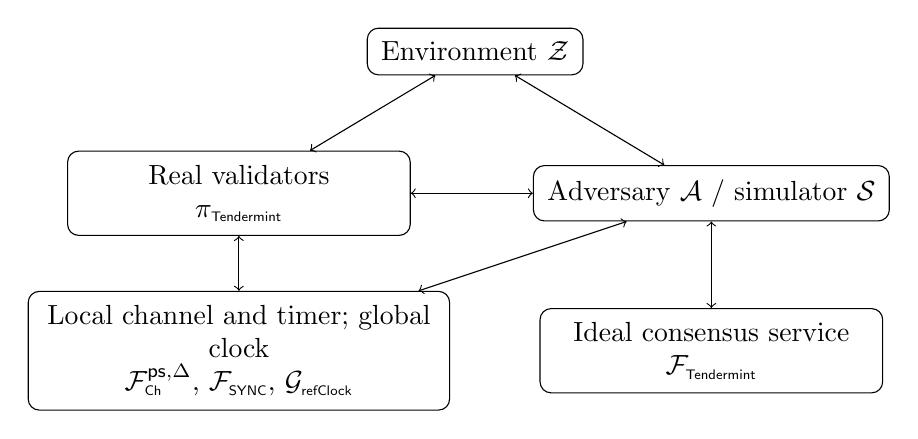
\begin{tikzpicture}[every node/.style={draw,rounded corners,align=center,inner sep=5pt}]
  \node (env) at (0,2.0) {Environment $\mathcal{Z}$};
  \node (real) at (-3,0.2) {\parbox{4cm}{\centering Real validators\par $\pi_{\scriptscriptstyle\mathsf{Tendermint}}$}};
  \node (adv) at (3,0.2) {Adversary $\mathcal{A}$ / simulator $\mathcal{S}$};
  \node (task) at (3,-1.8) {\parbox{4cm}{\centering Ideal consensus service\par $\mathcal{F}_{\scriptscriptstyle\mathsf{Tendermint}}$}};
  \node (setup) at (-3,-1.8) {\parbox{5cm}{\centering Local channel and timer; global clock\par $\mathcal{F}_{\scriptscriptstyle\mathsf{Ch}}^{\mathsf{ps},\Delta}$, $\mathcal{F}_{\scriptscriptstyle\mathsf{SYNC}}$, $\mathcal{G}_{\scriptscriptstyle\mathsf{refClock}}$}};
  \draw[<->] (env) -- (real);
  \draw[<->] (env) -- (adv);
  \draw[<->] (real) -- (adv);
  \draw[<->] (adv) -- (task);
  \draw[<->] (real) -- (setup);
  \draw[<->] (adv) -- (setup);
\end{tikzpicture}
\caption{Resource interfaces in the real and ideal worlds. Only the reference clock is global; channel and timer instances are session-local hybrids, simulated internally in the ideal world.}
\label{Tendermint-framework}
\end{figure*}

Let $V$ be the validator set at height $h$, with positive voting weights $w_i$ and total weight $W=\sum_{i\in V}w_i$. For $X\subseteq V$, write $w(X)=\sum_{i\in X}w_i$; let $C$ be the static corrupted set and $W_B=w(C)$. The weights remain fixed for all rounds at height $h$; any stake update is part of the public configuration for a later height. A quorum is a set $Q\subseteq V$ with $w(Q)>2W/3$. The public configuration fixes a deterministic proposer schedule $\mathsf{proposer}(h,r)$ consistent with the weighted rotation abstraction of the cited specification. Voting power remains fixed within a height; changing proposer priority is not stake redistribution. The implementation-specific priority normalization is not needed for the arguments below. Any recurrence used to derive a quantitative fairness bound requires its own specification and proof~\cite{buchman2018latest}.

\subsection{Supporting Functionalities}

Only $\mathcal{G}_{\scriptscriptstyle\mathsf{refClock}}$ is global. The communication resource $\mathcal{F}_{\scriptscriptstyle\mathsf{Ch}}^{\mathsf{ps},\Delta}$ and timer resource $\mathcal{F}_{\scriptscriptstyle\mathsf{SYNC}}$ are session-local hybrids. Their interfaces bind each request to its actual caller and $sid$; the simulator executes local copies internally and does not impersonate honest owners at a global resource.

\paragraph{Public authenticated communication.}
$\mathsf{Send}(sid,j,m)$ from $i$ creates a fresh delivery identifier and discloses $(sid,i,j,m)$ to the scheduler. Delivery returns the original sender and unchanged message. For forwarded votes, authentication must preserve the \emph{originator}, not merely the last forwarding peer: the abstraction permits forwarding an existing authenticated record but never creating a record attributed to an honest validator that did not issue it. This is an ideal transferable-authentication assumption; hop authentication alone would not suffice for PoLC evidence. No concrete signature realization is proved here. The scheduler may reorder, delay, or drop traffic before GST. For liveness, the communication resource additionally satisfies the gossip dissemination premise of the cited protocol: a message sent or received by an honest validator at time $t$ reaches all honest validators by $\max\{t,\mathsf{GST}\}+\Delta$~\cite{buchman2018latest}. This premise includes buffered evidence and is stronger than timely point-to-point delivery alone. It does not require Byzantine senders to broadcast consistently. GST and $\Delta$ need not be known to validators.

\paragraph{Reference time and local timers.}
The reference clock has an initially zero integer counter, increased by one on $\mathsf{IncrementTime}$ from the environment. Its public $\mathsf{GetTime}$ interface returns the counter; querying is distinct from advancing time~\cite{canetti2017universally}. We use exact relative timers, without claiming tolerance of approximate-clock drift. Retaining the original time-management commands, let $tag=(h,r,phase,k)$ include a generation number $k$. On $\mathsf{TimeStart}(sid,tag,T)$ from owner $p$, the local timer records $(p,sid,tag,G_{start},T)$ after querying the clock. On $\mathsf{IsTimeout}(sid,tag)$ from that owner, it queries the clock again and returns $\mathsf{TimeOut}$ iff $G-G_{start}\geq T$, otherwise $\mathsf{TimeRemain}$. $\mathsf{ResetTime}$ cancels that record; replies for old generations have no effect. Below, $\mathsf{StartTimer}$ and $\mathsf{CancelTimer}$ denote these start and reset operations, and $\mathsf{TimerExpired}$ denotes processing a matching $\mathsf{TimeOut}$ reply. It is not an unsolicited interrupt from the reference clock.

An adversarial $\mathsf{Sleep}/\mathsf{Wake}$ schedules an activation or reply; it neither changes elapsed time nor certifies that a timeout has occurred. Unrestricted schedules may withhold activations. Liveness therefore additionally requires time to increase without bound, pending honest communication to receive its stipulated service, and honest validators to receive enough activations to poll and process enabled transitions. A numerical reference-time bound also requires a bound on these service delays, included in the processing budget. Clock progress alone does not provide this service guarantee~\cite{katz2013universally}. The delayed-clock functionality in~\cite{canetti2017universally} is not invoked as a guaranteed-wakeup primitive.

\subsection{Ideal Functionality \texorpdfstring{$\mathcal{F}_{\scriptscriptstyle\mathsf{Tendermint}}$}{F-Tendermint}}

We retain the original operational organization of one functionality: proposal management, voting/decision, and time administration. The functionality maintains abstract validator states and authenticated message records, rather than network packets or a concrete signature algorithm. Its external contract is agreement and application validity in every execution, and the conditional progress statement below for admissible timed executions. The protocol-state guards constrain the simulator's choices; they are not commands permitting it to assign honest locks or votes.

\begin{myframebox}[title={ $\mathcal{F}_{\scriptscriptstyle\mathsf{Tendermint}}$: height and proposal management}]
\textbf{Initialization.} Fix $(sid,h,V,(w_i),C,\mathsf{Valid}_h)$ publicly, with $C$ static. For each honest validator initialize the height, round, phase, lock/valid pairs, message buffers, sent-vote flags, timer records, and a private candidate queue according to the real protocol specification below. All state is indexed by $sid$ and height. A new round retains height-local locks and evidence; a new height uses its public configuration and resets height-local state.

\textbf{Private input.} An honest input $\mathsf{Propose}(sid,h,v)$ appends $v$ to the owner's private candidate queue. Only receipt metadata $(sid,h,p,k)$, with input index $k$, is disclosed. The real candidate interface exposes exactly this metadata to its scheduler. Candidate contents and validity results are not disclosed at receipt. Fresh candidates are consumed in input order only when the selected proposer is ready to broadcast; an existing valid value has priority. Liveness requires valid candidates to be available when needed. Private application computations beyond this interface are outside the model.

\textbf{Proposal publication.} An activation of the selected proposer executes its enabled proposal rule using its stored state and candidate. Only the resulting proposal broadcast reveals the block and its evidence to the simulator. Record the broadcast as a fresh authenticated message identifier. Reproposing a public valid value causes no new private-input disclosure. The simulator cannot request the contents of an unused candidate independently of this transition.
\end{myframebox}

\begin{myframebox}[title={ $\mathcal{F}_{\scriptscriptstyle\mathsf{Tendermint}}$: voting and decision}]
\textbf{Message records.} A record contains $(sid,h,origin,r,phase,value,evidence)$ and its intended recipients. Honest records are created only by the functionality's enabled honest transitions. The simulator may inject arbitrary records attributed to members of $C$, but cannot create an honest-origin record. Reforwarding preserves the original record and origin. Invalid, wrong-session, and malformed evidence cannot satisfy an honest voting guard.

\textbf{Delivery and transition.} On $\mathsf{Deliver}(id,p)$ from the simulator, require an existing record addressed to $p$ and place it in $p$'s buffer. On $\mathsf{Activate}(p)$, process the next enabled local transition, using Algorithm~1 of~\cite{buchman2018latest} and the operational guards below. Fix the same tie-breaking order for simultaneously enabled transitions in the real and ideal machines. Count unique origins separately for each round, phase, and value; ordinary reception alone does not advance a phase. All honest sends are disclosed as new records. The simulator chooses the schedule, not the honest vote, lock, or valid-value assignment. Corrupted proposals enter through injection and delivery, without requiring an honest candidate-input submission.

\textbf{Decision.} A valid proposal and matching precommit quorum enable an honest output $\mathsf{Output}(h,v)$. Record that party's decision once. Fix the height's output value on its first decision and reject a conflicting output; the safety argument below shows this rejection is unreachable on valid transitions. No independent simulator command can select a decision value or release an unsupported output. Retain decision evidence for dissemination to lagging honest validators.
\end{myframebox}

\begin{myframebox}[title={ $\mathcal{F}_{\scriptscriptstyle\mathsf{Tendermint}}$: administration and time}]
\textbf{TimeStart/ResetTime.} An enabled protocol rule starts or cancels its timer, keyed by owner, session, height, round, phase, and generation. On start, query the actual $\mathcal{G}_{\scriptscriptstyle\mathsf{refClock}}$ and record the duration and start time. The simulator cannot reset or shorten an honest timer independently of a protocol transition.

\textbf{Sleep/Wake and IsTimeout.} Pending local work may wait for a scheduler activation. $\mathsf{Wake}(p)$ is an alias for $\mathsf{Activate}(p)$, not permission to change elapsed time. To process a timer, query $\mathsf{GetTime}$ and apply the same expiration test as the local timer interface. Stale generations do nothing. A timeout can act only when both its duration and activation conditions hold.

\textbf{Scheduling contract.} In unrestricted executions the simulator may withhold service, and no unconditional termination is promised. An admissible timed execution supplies the stipulated gossip delivery and honest activation service; it cannot indefinitely withhold a required delivery or wakeup. Section~\ref{sec:protocol} states the additional proposer/evidence and timeout premises and derives the corresponding decision bound. Time advance belongs exclusively to the environment. These are execution conditions, not secret knowledge of GST supplied to honest parties.
\end{myframebox}

\section{Real World, Simulator, and Security Proof}\label{sec:protocol}

We analyze the abstract Tendermint state machine over the local hybrids and global clock defined in Section~\ref{sec:model}. The GUC statement below is a security and simulation statement. The post-GST liveness result is proved separately and has explicit assumptions on time progress, the current round, and proposer fairness.

\subsection{Formal Protocol Specification}

The real protocol $\pi_{\scriptscriptstyle\mathsf{Tendermint}}$ is the abstract consensus state machine in Algorithm~1 of arXiv:1807.04938v3~\cite{buchman2018latest}; we do not claim to verify a particular ChainMaker release. At each height, $\mathsf{NEWHEIGHT}$ initializes the height-local state and $\mathsf{NEWROUND}$ advances the round. These are management transitions. The three voting phases are Propose, Prevote, and Precommit. A validator prevotes for a valid proposal when its lock rule permits it, otherwise it may prevote $\mathsf{nil}$. A prevote quorum of weight greater than $2W/3$ updates the validator's valid-value and PoLC information and permits a precommit according to the locking rule. A precommit quorum of weight greater than $2W/3$ causes a local decision; there is no fourth voting phase called Commit. Each honest validator keeps its own $(\mathsf{lockedValue},\mathsf{lockedRound})$ and $(\mathsf{validValue},\mathsf{validRound})$. The functionality tracks their abstract counterparts, and the proof relates these states event by event.

\paragraph{Operational guards retained from the original model.}
The following makes the original NewRound, voting, and time-management organization explicit. The complete transition ordering is Algorithm~1 of~\cite{buchman2018latest}; the rules below specify its interface translation, not an alternative consensus algorithm.
\begin{enumerate}
\item At a new height initialize both lock and valid-value pairs to $(\mathsf{nil},-1)$. A new round resets phase-local flags and timers, but preserves both pairs and buffered evidence for this height. The proposer uses its valid value when available, otherwise a valid application candidate.
\item Cache authenticated messages by $(sid,h,r,phase,value,origin)$. Count each origin once in a tally; distinct values have distinct tallies. A phase-wide quorum over mixed values uses the union of origins, never the sum of per-value tallies. Receiving a vote alone does not advance the phase. Honest validators issue at most one prevote and one precommit per round. Quorum guards use weight strictly greater than $2W/3$.
\item In Propose, prevote a valid proposal when the lock/evidence guard above holds; otherwise follow the specification's nil-vote and proposal-timeout rules. Evidence for a nonnegative $vr$ must be for the same height and value. Retain late evidence so that a previously unsatisfied guard can become enabled.
\item A valid proposal and a matching current-round prevote quorum update $(\mathsf{validValue},\mathsf{validRound})$. If still in Prevote, also set $\mathsf{lockedValue}=v$ and $\mathsf{lockedRound}=r$, then precommit $v$. A nil quorum or the applicable prevote timeout can cause a nil precommit, but does not create a block lock. The prevote timeout starts on sufficient current-round prevotes, including votes for different values, as specified by the original algorithm; it does not start merely on phase entry.
\item A valid proposal together with its matching precommit quorum permits a decision once per height, including when the decision evidence is for an earlier round. Sufficient current-round precommits start the precommit timer; expiration enters the next round. Separately, messages from distinct origins of weight greater than $W/3$ in one higher round permit catching up to that round. This threshold establishes honest participation; it is not a decision quorum.
\end{enumerate}

\begin{lemma}[Execution correspondence]\label{lem:execution-correspondence}
For the protocol defined by Algorithm~1 with the interface translation above, erase session tags, local resource calls, and reference-time queries from a real hybrid execution, retaining authenticated protocol messages, timer expirations, local state changes, and outputs. The resulting trace is an execution of the cited Tendermint transition system. In its zero-local-time timing specialization, with the stipulated gossip, timeout, activation, and proposer premises, the referenced termination argument applies to this trace.
\end{lemma}
\begin{proof}
Induct on protocol transitions. Initialization and new-round transitions preserve the same state variables. A resource delivery supplies the original authenticated message; forwarding does not change its origin, and duplicate suppression preserves vote sets. The proposal, quorum, lock, and catch-up guards are precisely the guards of the cited algorithm with thresholds expressed in voting weight. Timer polling cannot expire a timer before its recorded duration; cancellation prevents an old timer from acting in a new round. Erased polling and resource bookkeeping are stuttering steps, while an enabled timeout performs the same algorithmic transition. Thus each retained transition is legal and preserves the state and decision mapping. For the timed specialization, the gossip resource supplies the source model's delivery premise, and the activation and timeout premises supply its timing behavior. Applying its termination proof consequently requires no independent reproof of the consensus algorithm. Positive processing costs require an additional timing adaptation; this lemma does not establish a new quantitative bound for them.
\end{proof}

This correspondence concerns the \emph{real protocol}. The simulation proof additionally establishes that its outputs pass the ideal consistency guard. Progress of either machine requires the stated scheduling premises, rather than the mere existence of a simulator.

\subsection{Designing the Simulator}\label{subsec:simulator}

The simulator $\mathcal{S}$ runs $\mathcal{A}$ internally and emulates the session-local channel and timer interfaces. The single reference clock remains external. It also tracks the public part of the honest protocol states, with opaque entries for unpublished candidates. Its event handling follows the internal-execution method of~\cite{canetti2017universally}:
\begin{enumerate}
\item \textbf{Initialization and inputs.} Initialize public configuration and the fixed corruption set. Forward only the candidate-receipt metadata that the real interface exposes. The ideal functionality retains the private candidate contents; the simulator neither reads nor guesses them.
\item \textbf{Honest activation and publication.} Map an honest scheduling activation to $\mathsf{Activate}(p)$. The functionality executes the corresponding enabled rule. At an honest broadcast it supplies the resulting authenticated record, including a fresh candidate only when published. Use this record to complete the matching internal send and give $\mathcal{A}$ the same sender, recipients, and payload as the real local channel would reveal. The record is an adversarial notification, not an extra output to the environment.
\item \textbf{Corrupted messages and delivery.} Forward $\mathcal{A}$'s corrupted-origin injections; internally maintain the channel queue. On a scheduled delivery, submit the matching record identifier and recipient to the functionality. A forwarded honest record must already exist. Duplicate packets can be scheduled but cannot add voting weight. The same before/after-GST scheduling restrictions apply to the paired executions.
\item \textbf{Time and local state.} Emulate local timer queries using public $\mathsf{GetTime}$ as needed and schedule the corresponding ideal activation. Both machines apply the same expiration test and generation check. Honest lock and PoLC updates are computed by their transition rules, not written at the simulator's request. Neither the simulator nor the functionality advances the global clock.
\item \textbf{Decision and surrounding execution.} When the corresponding precommit guard becomes enabled, the functionality produces the matching honest output. Forward communications between $\mathcal{A}$ and the environment, preserving session identifiers and message order. Unrelated sessions retain their actual global resource access; the simulator does not inspect their private state.
\end{enumerate}

The construction is event-driven: it simulates only scheduled transitions, with polynomial overhead in the execution prefix, rather than busy-waiting for time to advance. Transferable authentication is ideal in this model; no concrete signature reduction or adaptive-corruption claim is made.

\subsection{Ideal-Real Mapping}

\begin{lemma}[Weighted quorum intersection]\label{lem:weighted-intersection}
If $Q_1,Q_2\subseteq V$ both have weight greater than $2W/3$, then $w(Q_1\cap Q_2)>W/3$. In particular, if Byzantine voting weight is $W_B<W/3$, their intersection contains positive honest voting weight.
\end{lemma}
\begin{proof}
$w(Q_1\cap Q_2)=w(Q_1)+w(Q_2)-w(Q_1\cup Q_2)\geq w(Q_1)+w(Q_2)-W>W/3$. Since $w(C)<W/3$, the intersection cannot consist only of corrupted validators.
\end{proof}

\begin{lemma}[Agreement and validity of guarded executions]\label{lem:guarded-safety}
With $W_B<W/3$, the real transition system and the operational functionality produce only valid, nonconflicting honest decisions at a fixed height.
\end{lemma}
\begin{proof}
A decision of $v$ in round $r$ includes a precommit quorum. Its honest precommitters have weight greater than $W/3$ and each locked $v$ in that round. A conflicting prevote quorum in the same round is impossible because the prevote quorum supporting those precommits intersects it in an honest origin, which votes once. Suppose a conflicting prevote quorum exists in a later round and choose its smallest round index $r'$. It intersects the honest locked set. An honest member could vote for that conflicting value only with a matching earlier PoLC whose round is at least its lock round. Such evidence either contradicts same-round quorum intersection at $r$, or is a conflicting quorum between $r$ and $r'$, contrary to minimality. Locks persist across rounds, and nil does not erase them. Thus no first conflicting quorum exists. Any conflicting decision would require one, since its precommit quorum contains an honest precommitter. Proposal validity is checked before a block vote or decision. The same reasoning applies to the ideal transition rules without invoking the extra output-consistency check. This is the weighted form of the cited lock-safety argument.
\end{proof}

\paragraph{Interface scope.}
The candidate interface exposes only receipt metadata before proposal publication; unpublished values cannot influence earlier consensus control transitions. The statement concerns this specified interface and the ideal transferable-authentication hybrid, not arbitrary application-side leakage or concrete cryptographic implementations.

\begin{theorem}[GUC simulation for the abstract protocol]\label{thm:tendermint-mapping}
Fix the global setup $\mathcal{G}=\mathcal{G}_{\scriptscriptstyle\mathsf{refClock}}$ and the session-local $(\mathcal{F}_{\scriptscriptstyle\mathsf{Ch}}^{\mathsf{ps},\Delta},\mathcal{F}_{\scriptscriptstyle\mathsf{SYNC}})$ hybrid and a public height configuration with $w(C)<W/3$. For every PPT adversary $\mathcal{A}$ whose corruption set $C$ is fixed before the session, there is a PPT simulator $\mathcal{S}$ such that for every allowed PPT GUC environment $\mathcal{Z}$,
\[
\mathsf{GEXEC}_{\mathcal{G},\pi_{\scriptscriptstyle\mathsf{Tendermint}},\mathcal{A},\mathcal{Z}}
\approx
\mathsf{GEXEC}_{\mathcal{G},\mathcal{F}_{\scriptscriptstyle\mathsf{Tendermint}},\mathcal{S},\mathcal{Z}}.
\]
This is a statement in the abstract authenticated-message hybrid model. It makes no claim about realization of the shared resources from concrete cryptographic or network implementations.
\end{theorem}

\begin{proof}
Couple the real and ideal public configuration, corrupted actions, scheduled activations, and protocol randomness. Candidate inputs are supplied to the real validator or its ideal counterpart, respectively. Maintain the following relation after every protocol event: honest consensus states and private candidate queues agree; authenticated record sets and delivery buffers agree up to record-identifier renaming; timers have the same start times, durations, and generations; and honest outputs and adversarial notifications agree. The simulator knows only the public projection of this relation, not unpublished candidate values.

Initialization establishes the relation. An input appends the same private value and exposes the same receipt metadata. On activation, the two machines use the same enabled rule and tie-breaking order. A fresh proposal is computed from equal private queues or an equal existing valid value; its publication therefore gives the simulator precisely the real broadcast payload. Corrupted injection and scheduled delivery preserve origin and content, and unique-origin counting gives equal quorum tests. Polling uses the same global time and timer record. Local bookkeeping may add internal activations, but it does not advance the clock or create an additional externally visible message. These cases preserve the relation through each send, lock update, timeout, and round transition.

At a real decision, the same valid proposal and precommit quorum are present in the ideal state. Such a proposal may originate from either an honest publication or a corrupted injection; there is no missing candidate-registration prerequisite. Lemma~\ref{lem:guarded-safety}, together with the execution correspondence, excludes a conflicting honest decision. Validity comes from the real proposal/decision guards. Thus the ideal consistency guard never suppresses a real output; it is not used as a circular proof of protocol safety.

Local hybrid resources are simulated internally, while every global reference-time query refers to the actual shared clock. No global state is cloned or programmed. Session-local bookkeeping leaves unrelated executions unchanged. The environment receives the same honest outputs and the same forwarded adversarial communications; hence the coupled finite view prefixes coincide. With ideal authentication this gives identical view distributions, and therefore the stated indistinguishability. Timing admissibility is not needed for this safety/view correspondence; when imposed for liveness it must hold in both executions.
\end{proof}

\subsection{Proof of the Termination Bound}

We retain the original distinction between a successful round, unsuccessful rounds, and their cumulative cost. Time below is the public reference time; validators use local timers. Let $D$ be the post-GST gossip bound. In the exact-timer, zero-local-processing specialization of the cited protocol, $D=\Delta$. In this specialization, enabled honest transitions and due timer polls are serviced at their reference time before the next clock increment; merely receiving infinitely many activations would not suffice for a numerical bound. This specialization permits direct reuse of its progress lemmas~\cite{buchman2018latest}. A positive processing bound $\delta$ by itself does not justify replacing every occurrence of $D$ by $\Delta+\delta$: one must also bound activation, polling, and the number of sequential processing steps. The numerical theorem here is stated for the specialization; the general processing-cost extension remains outside this bound.

Write $P_r,V_r,C_r$ for the Propose, Prevote, and Precommit timeout durations. They are configured protocol parameters, not measurements of adversarial delay. Use integer reference-time units and integer timeout parameters. Linear timeouts have the form $X_r=a_X+r b_X$ for $X\in\{P,V,C\}$. For all rounds used below require
\[
 P_r>2D+C_{r-1},\qquad V_r>2D,\qquad C_r>2D.
\]
The protocol need not know GST or $D$. For example, positive slopes with $b_P>b_C$ and $b_V,b_C>0$ eventually meet these inequalities for every fixed $D$. Equal positive slopes alone need not make the first inequality eventually true. Timeout counters do not reset at GST.

\paragraph{Successful round without timeout-driven failure.}
Let $t_r>\mathsf{GST}$ be the first honest entry into a fresh round $r>0$. Assume an honest proposer whose valid-round information covers the honest locks at that point, with the matching value and evidence available under the protocol rules. Lemma~5 of~\cite{buchman2018latest}, applied through Lemma~\ref{lem:execution-correspondence}, gives
\[
 T_{\mathrm{dec}}\leq t_r+4D+C_{r-1}.
\]
The $C_{r-1}$ term covers entry skew; honest validators need not enter together. The timeout inequalities and gossip premise establish timely proposal and vote delivery. Timely completion is a conclusion of this argument, not part of the definition of a good round. Actual adversarial network delay is included in $D$, rather than silently set to zero.

\begin{lemma}[Cost of an unsuccessful round]\label{lem:failed-round}
In the same timing specialization, after first honest entry at $t_r>\mathsf{GST}$ into a fresh round $r$ above all rounds entered by honest validators at GST, either a decision certificate disseminates, or the next first honest entry occurs by
\[
 t_{r+1}\leq t_r+B_r,\qquad
 B_r=C_{r-1}+P_r+V_r+C_r+3D.
\]
\end{lemma}
\begin{proof}
The first honest entry into a previously unentered round cannot be justified solely by higher-round Byzantine messages: their weight is below the catch-up threshold. It originates in the preceding round's precommit-timer expiration. The precommits that started that timer disseminate within $D$; honest laggards can catch up and finish that preceding timer. Hence every still-undecided honest validator reaches round $r$ by $e_r=t_r+D+C_{r-1}$, unless progress beyond that round has already occurred.

If no honest validator has yet left round $r$, by $e_r+P_r$ each has prevoted, using nil on proposal timeout if necessary. Their aggregate weight exceeds $2W/3$. These votes reach all honest validators within $D$, enabling the prevote timeout even when values differ. Thus each has precommitted a value or nil by $e_r+P_r+D+V_r$. Another dissemination interval enables the precommit timeout, and its expiration advances the round by $e_r+P_r+D+V_r+D+C_r$. This is $t_r+B_r$. If an honest validator advances earlier, the required first-entry bound already holds. If an honest validator decides earlier, its proposal and precommit certificate disseminate within $D$ and permit the other honest decisions irrespective of their current round. No estimate in this argument treats a quorum-triggered timer as if it started on phase entry.
\end{proof}

\begin{theorem}[Conditional post-GST liveness]\label{thm:conditional-liveness}
Assume $W_B<W/3$, exact timers, zero local processing time and the immediate activation service defined above, the gossip bound $D$, and valid application candidates when requested. Let $t_s>\mathsf{GST}$ be the first honest entry into a fresh round $r_s>0$ above all honest rounds at GST, with the timeout inequalities holding from that round onward. Suppose among $r_s,\ldots,r_s+L$ there is an honest-proposer round with the lock/evidence condition of the successful-round argument. Then all honest validators decide the same valid value, and
\[
 T^*\leq t_s+\sum_{r=r_s}^{r_s+L-1}B_r
                 +4D+C_{r_s+L-1}.
\]
An empty sum is zero. For nonnegative linear increments, write
\[
 \begin{aligned}
 B_r&=A+rB,\\
 A&=a_P+a_V+2a_C-b_C+3D,\\
 B&=b_P+b_V+2b_C.
 \end{aligned}
\]
Consequently the failed-round sum is
\[
 LA+B\left(Lr_s+\frac{L(L-1)}2\right).
\]
\end{theorem}
\begin{proof}
If the first successful round is $r_s+j$ with $0\leq j\leq L$, apply Lemma~\ref{lem:failed-round} to each preceding round and then the successful-round bound. An earlier decision certificate only shortens the execution: its remaining dissemination cost is at most $D$. Nonnegative timeout increments permit replacing $j$ by $L$ for an upper bound. Summing the affine $B_r$ gives the expression. Agreement and validity are inherited from the protocol correspondence and weighted quorum argument, independently of this timing calculation.
\end{proof}

\paragraph{Fairness, inherited termination, and scope.}
The parameter $L$ bounds the wait for an honest proposer with the required lock evidence; it does not assume that voting has already succeeded. The cited lock-propagation and termination arguments (Lemmas~6--7) explain how their scheduling and gossip premises supply such progress. To inherit those conclusions, the corresponding premises must hold in the UC execution. We do not infer a uniform numerical $L$ from arbitrary stake distributions, or identify it with the number of corrupted validators. If timeout coefficients are $O(D)$, the displayed bound is $t_s+O((L+1)(r_s+L+1)D)$. Replacing $t_s$ by GST or removing $r_s$ requires additional bounds; neither follows from UC composition. This formulation avoids an unproved simultaneous-entry parameter $T_{\mathsf{align}}$.

The GUC replacement guarantee concerns the properties actually imposed by the ideal interface and its shared setup. A terminating-service composition theorem additionally requires an ideal progress contract and preservation of the resource/activation premises in the higher-level execution~\cite{katz2013universally,canetti2017universally}. The operational functionality imposes the same honest guards and timed scheduling contract. Applying the same execution correspondence to an admissible ideal trace yields the same conditional bound for the ideal service. Consequently its use under composition requires preservation of these premises; no unconditional guarantee is asserted for a higher-level environment that withholds time or required activations.

\section{TLA+ Verification of Functionality\label{sec:tla+}}

We use TLA+ to formally assess whether $\mathcal{F}_{\scriptscriptstyle \mathsf{Tendermint}}$ terminates under bounded delay attacks. Agreement is checked as a supporting invariant throughout the analysis. The TLA+ specification is publicly available\footnote{\url{https://anonymous.4open.science/r/UC-tla-102E/}}. We use Apalache~\cite{konnov2019tla+}, a Satisfiability Modulo Theories (SMT)-based model checker that supports bounded checking, which is exhaustive up to a fixed trace length, and simulation, which generates randomized traces to probe complementary parts of the state space.

\subsection{TLA+ modeling of the ideal protocol}

\begin{figure}[!htbp]
  \centering
  \includegraphics[width=\linewidth]{figures/Tendermint-TLA+-Framework-new.png}
  \caption{TLA$^+$ modeling of the Tendermint protocol workflow.}
  \label{Tendermint-tla+-framework}
\end{figure}

The ideal protocol is modeled using a three-layer architecture (Fig.~\ref{Tendermint-tla+-framework}). The global environment layer abstracts $\mathcal{G}_{\scriptscriptstyle \mathsf{refClock}}$, $\mathcal{F}_{\scriptscriptstyle \mathsf{BC}}$, and $\mathcal{F}_{\scriptscriptstyle \mathsf{SYNC}}$, and advances time through $\texttt{ClockTick}$. The validator layer records $h_p$, $round_p$, $phase_p$, and $lockedValue_p$, with the transition sequence $\texttt{NewRoundAndPropose} \to \texttt{Prevote} \to \texttt{Precommit} \to \texttt{Commit}$. For verification efficiency, the five-phase protocol is represented as four phases by merging NewRound and Propose. The adversary layer models corruption and delay attacks through $\texttt{AdversaryWake}$, which gives the scheduler fine-grained control over honest-node timing.

\subsection{Termination verification}

We verify termination of $\mathcal{F}^{V,\Delta,\Sigma}_{\mathrm{Tendermint}}$ under bounded delay attacks using two complementary Apalache workflows~\cite{konnov2019tla+}. The first performs exhaustive bounded checking of the full interleaved specification. The second uses a coalesced honest-transition path that reduces state-space growth from $O(|V|^k)$ to $O(|V|\cdot H_{\max}\cdot R_{\max})$. Both workflows check the same termination predicate and agreement invariant, allowing the scalable mode to extend the bounded analysis to larger validator sets.

\begin{table*}[!t]
\centering
\caption{
Verification results for $\mathcal{F}^{V,\Delta,\Sigma}_{\mathrm{Tendermint}}$ under bounded delay attacks.
The exhaustive mode ($|V|=4$, $f=1$, $H_{\max}=1$) explores parameter sensitivity across
$\Sigma\times\Delta\times R_{\max}$ with aggressive values ($\Sigma\in\{3,4,5\}$, $\Delta\in\{3,4\}$).
The scalable mode evaluates larger validator sets with $|V|\in\{7,10,13\}$ and $H_{\max}\in\{3,5\}$.
All checks evaluate the \texttt{Agreement} and \texttt{NotYetTerminated} invariants.
}
\label{tab:comprehensive}
\resizebox{\textwidth}{!}{
\setlength{\tabcolsep}{3pt}
\begin{tabular}{lccrrrrrrc}
\toprule
\textbf{Mode} & \textbf{Check} & $|V|$ & $f$ & $H_{\max}$ &
   $\Sigma/\Delta$ & $R_{\max}$ & \textbf{len} & \textbf{Time(s)} & \textbf{Result} \\
\midrule
1  & standard        &  4 & 1 & 1 & 3/3 & 2 & 5 & 30.3 & PASS \\
1  & standard        &  4 & 1 & 1 & 3/3 & 3 & 5 & 26.9 & PASS \\
1  & standard        &  4 & 1 & 1 & 3/3 & 5 & 5 & 27.6 & PASS \\
1  & standard        &  4 & 1 & 1 & 4/3 & 2 & 5 & 25.9 & PASS \\
1  & standard        &  4 & 1 & 1 & 4/3 & 3 & 5 & 28.5 & PASS \\
1  & standard        &  4 & 1 & 1 & 4/4 & 3 & 5 & 25.7 & PASS \\
1  & standard        &  4 & 1 & 1 & 5/4 & 3 & 5 & 26.0 & PASS \\
\midrule
2  & optimized-attack-agreement        &  7 & 2 & 5 & 1/1 & 2 & 30 & 74.7 & PASS \\
2  & optimized-attack-termination      &  7 & 2 & 5 & 1/1 & 2 & 30 & 58.0 & PASS \\
2  & optimized-attack-agreement        &  7 & 2 & 5 & 1/1 & 3 & 30 & 71.3 & PASS \\
2  & optimized-attack-termination      &  7 & 2 & 5 & 1/1 & 3 & 30 & 54.1 & PASS \\
2  & optimized-attack-agreement        &  7 & 2 & 3 & 1/1 & 2 & 22 & 43.4 & PASS \\
2  & optimized-attack-termination      &  7 & 2 & 3 & 1/1 & 2 & 22 & 30.9 & PASS \\
2  & optimized-attack-agreement        &  7 & 2 & 3 & 1/1 & 5 & 22 & 42.9 & PASS \\
2  & optimized-attack-termination      &  7 & 2 & 3 & 1/1 & 5 & 22 & 29.3 & PASS \\
2  & optimized-attack-agreement        & 10 & 3 & 3 & 1/1 & 3 & 24 & 98.3 & PASS \\
2  & optimized-attack-termination      & 10 & 3 & 3 & 1/1 & 3 & 24 & 72.6 & PASS \\
2  & optimized-attack-agreement        & 13 & 4 & 3 & 1/1 & 3 & 26 & 37.0 & PASS \\
2  & optimized-attack-termination      & 13 & 4 & 3 & 1/1 & 3 & 26 & 24.5 & PASS \\
\bottomrule
\end{tabular}
}
\end{table*}
\subsubsection{Aggressive parameter sweep.}

The exhaustive checks in Table~\ref{tab:comprehensive} fix $V=\{v_1,v_2,v_3,v_4\}$ ($f=1$, $H_{\max}=1$) and vary $\Sigma\in\{3,4,5\}$ and $\Delta\in\{3,4\}$. These settings stress the attack guard $\mathrm{DelayAttack}(p): (\delta+\sigma_p>2\Delta)\vee(\sigma_p>2\Sigma)$ and measure degraded protocol steps, including nil votes and round advances without decision. Termination is evaluated using:
\[
\begin{aligned}
 &\mathsf{NotYetTerminated} \triangleq{}\\
 &\quad\lnot\big(\forall p\in InitiallyHonest:\\
 &\qquad decision[p][0]\neq NilValue\big).
\end{aligned}
\]
Agreement is checked as a supporting invariant:
\begin{multline*}
\mathsf{Agreement} \triangleq \forall \ell\in 0..\mathsf{MaxHeight},\;
\forall p,q\in \mathsf{InitiallyHonest}:\\
\bigl(decision[p][\ell]\neq \mathsf{NilValue} \land
decision[q][\ell]\neq \mathsf{NilValue}\bigr)\\
\;\Rightarrow\; decision[p][\ell]=decision[q][\ell].
\end{multline*}
All seven runs across $R_{\max}\in\{2,3,5\}$ pass. A termination witness (Apalache RC$=12$) further confirms that every honest validator decides at height $0$ within the bounded horizon.

\subsubsection{Scalable verification.}

The scalable checks in Table~\ref{tab:comprehensive} fix $\Sigma=\Delta=1$ and evaluate $|V|\in{7,10,13}$, with $f=\lfloor(|V|-1)/3\rfloor$ and $H_{\max}\in{3,5}$. To control the $O(|V|^k)$ state-space growth of the interleaved specification, we use a coalesced honest transition that updates all honest validators in one step. This is sound under synchrony, where honest validators share the same height, round, and phase. It reduces growth to $O(|V|\cdot H_{\max}\cdot R_{\max})$ while preserving the four-phase core, quorum threshold, lock/unlock rules, $validValue$/$validRound$ propagation, and delay-attack semantics.

Across all 19 runs, including seven exhaustive delay-attack checks and 12 scalable checks over larger validator sets, the model checker returns PASS. Termination holds in every tested configuration, witness traces confirm bounded honest decisions, and the agreement invariant is always satisfied.

Together, exhaustive runs validate full interleaving semantics on the small configuration, while coalesced runs preserve the same safety and termination checks at scale. Thus, the checks provide a reproducible executable basis for the termination and agreement claims used in our UC analysis, without replacing an unbounded deductive proof.

\section{EasyUC}\label{sec:easyuc}

We mechanize the weighted quorum intersection argument in Lemma~\ref{lem:weighted-intersection} and the same-round agreement case of Lemma~\ref{lem:guarded-safety}. The EasyUC model describes voting at a fixed height and round. Its interpreter and the EasyCrypt proofs use the same transition function.

\subsection{Weighted Quorum Intersection}

We represent the finite validator set $V$ by a duplicate-free list and assign each validator a positive integer voting weight. For total weight $W=w(V)$, a quorum is a set $Q\subseteq V$ satisfying $3w(Q)>2W$. EasyCrypt proves the identity
\begin{equation*}
w(Q_1\cup Q_2)+w(Q_1\cap Q_2)=w(Q_1)+w(Q_2).
\end{equation*}
Since $w(Q_1\cup Q_2)\leq W$, two quorums satisfy $3w(Q_1\cap Q_2)>W$. The static Byzantine set $B$ satisfies $3w(B)<W$, so the intersection contains an honest validator.

\subsection{Same-Round Agreement}

The model records proposals, prevotes, precommits, and decisions. A delivery preserves the identity and contents of an existing publication. The scheduler may reorder or replay deliveries, and Byzantine validators may publish conflicting votes under their own identities. Each recipient counts the weight of distinct origins for a given phase and value.

An honest validator can publish a precommit for a proposed block after receiving a matching prevote quorum. The transition records the publication and disables further precommits by that validator. A decision requires a matching local precommit quorum. Induction over event sequences establishes that each recorded decision has a certificate and that honest validators publish at most one precommit. If two honest validators decide different blocks in the same round, the two certificates must share an honest origin by Lemma~\ref{lem:weighted-intersection}. That origin would have had to precommit both blocks, contradicting the precommit invariant. The theorem holds for any finite validator configuration satisfying the stated weight assumptions.

\subsection{Executable Verification}

The EasyUC interpreter checks a four-validator configuration with weights $(3,2,2,2)$, including one Byzantine validator of weight $2$. All three honest validators decide block $42$. Replaying a precommit of weight $3$ leaves the recipient's tally at $3$. The recipient cannot decide at weight $5$ and can decide at weight $7$. All 52 interpreter assertions pass. Section~\ref{sec:protocol} gives the cross-round lock argument, the GUC simulation, and the conditional termination proof.

\section{Conclusion}\label{sec:conclusion}

We specify an operational consensus functionality and give a GUC internal-simulation argument for the abstract Tendermint state machine in the stated authenticated-message hybrid model. Weighted quorum intersection together with the persistent-lock argument yields safety under static Byzantine voting weight below $W/3$. Separately, Theorem~\ref{thm:conditional-liveness} bounds latency in the exact-timer, zero-local-processing specialization using explicit lock-evidence fairness and the cost of starting quorum-triggered timers. The first sufficiently late round and its entry time remain in the bound; no simultaneous-entry assumption or GST reset is used. The analysis is discussed in relation to the public manuscript of Dong et al.~\cite{dong2025uctendermint}, with explicit operational modeling and proof conditions. The bounded TLA$^+$ section remains separate from these proofs.

Several directions merit future investigation. First, extending the numerical theorem to bounded positive processing and polling costs requires an explicit timing adaptation; heterogeneous communication bounds are another extension. Second, applying the UC+TLA+ methodology to other BFT protocols (e.g., HotStuff, Streamlet) would test its generalizability and potentially reveal protocol-specific attack surfaces. Third, integrating $\mathcal{F}_{\scriptscriptstyle \mathsf{Tendermint}}$ with higher-layer blockchain components such as mempools and cross-chain bridges would validate its robustness in fully composable real-world deployments.

\clearpage
\bibliographystyle{IEEEtran}
\bibliography{mybibliography}

\end{document}
